\documentclass[journal, a4paper]{IEEEtran}

% some very useful LaTeX packages include:

%\usepackage{cite}      % Written by Donald Arseneau
                        % V1.6 and later of IEEEtran pre-defines the format
                        % of the cite.sty package \cite{} output to follow
                        % that of IEEE. Loading the cite package will
                        % result in citation numbers being automatically
                        % sorted and properly "ranged". i.e.,
                        % [1], [9], [2], [7], [5], [6]
                        % (without using cite.sty)
                        % will become:
                        % [1], [2], [5]--[7], [9] (using cite.sty)
                        % cite.sty's \cite will automatically add leading
                        % space, if needed. Use cite.sty's noadjust option
                        % (cite.sty V3.8 and later) if you want to turn this
                        % off. cite.sty is already installed on most LaTeX
                        % systems. The latest version can be obtained at:
                        % http://www.ctan.org/tex-archive/macros/latex/contrib/supported/cite/

\usepackage{graphicx}   % Written by David Carlisle and Sebastian Rahtz
                        % Required if you want graphics, photos, etc.
                        % graphicx.sty is already installed on most LaTeX
                        % systems. The latest version and documentation can
                        % be obtained at:
                        % http://www.ctan.org/tex-archive/macros/latex/required/graphics/
                        % Another good source of documentation is "Using
                        % Imported Graphics in LaTeX2e" by Keith Reckdahl
                        % which can be found as esplatex.ps and epslatex.pdf
                        % at: http://www.ctan.org/tex-archive/info/

%\usepackage{psfrag}    % Written by Craig Barratt, Michael C. Grant,
                        % and David Carlisle
                        % This package allows you to substitute LaTeX
                        % commands for text in imported EPS graphic files.
                        % In this way, LaTeX symbols can be placed into
                        % graphics that have been generated by other
                        % applications. You must use latex->dvips->ps2pdf
                        % workflow (not direct pdf output from pdflatex) if
                        % you wish to use this capability because it works
                        % via some PostScript tricks. Alternatively, the
                        % graphics could be processed as separate files via
                        % psfrag and dvips, then converted to PDF for
                        % inclusion in the main file which uses pdflatex.
                        % Docs are in "The PSfrag System" by Michael C. Grant
                        % and David Carlisle. There is also some information
                        % about using psfrag in "Using Imported Graphics in
                        % LaTeX2e" by Keith Reckdahl which documents the
                        % graphicx package (see above). The psfrag package
                        % and documentation can be obtained at:
                        % http://www.ctan.org/tex-archive/macros/latex/contrib/supported/psfrag/

%\usepackage{subfigure} % Written by Steven Douglas Cochran
                        % This package makes it easy to put subfigures
                        % in your figures. i.e., "figure 1a and 1b"
                        % Docs are in "Using Imported Graphics in LaTeX2e"
                        % by Keith Reckdahl which also documents the graphicx
                        % package (see above). subfigure.sty is already
                        % installed on most LaTeX systems. The latest version
                        % and documentation can be obtained at:
                        % http://www.ctan.org/tex-archive/macros/latex/contrib/supported/subfigure/

\usepackage{url}        % Written by Donald Arseneau
                        % Provides better support for handling and breaking
                        % URLs. url.sty is already installed on most LaTeX
                        % systems. The latest version can be obtained at:
                        % http://www.ctan.org/tex-archive/macros/latex/contrib/other/misc/
                        % Read the url.sty source comments for usage information.

%\usepackage{stfloats}  % Written by Sigitas Tolusis
                        % Gives LaTeX2e the ability to do double column
                        % floats at the bottom of the page as well as the top.
                        % (e.g., "\begin{figure*}[!b]" is not normally
                        % possible in LaTeX2e). This is an invasive package
                        % which rewrites many portions of the LaTeX2e output
                        % routines. It may not work with other packages that
                        % modify the LaTeX2e output routine and/or with other
                        % versions of LaTeX. The latest version and
                        % documentation can be obtained at:
                        % http://www.ctan.org/tex-archive/macros/latex/contrib/supported/sttools/
                        % Documentation is contained in the stfloats.sty
                        % comments as well as in the presfull.pdf file.
                        % Do not use the stfloats baselinefloat ability as
                        % IEEE does not allow \baselineskip to stretch.
                        % Authors submitting work to the IEEE should note
                        % that IEEE rarely uses double column equations and
                        % that authors should try to avoid such use.
                        % Do not be tempted to use the cuted.sty or
                        % midfloat.sty package (by the same author) as IEEE
                        % does not format its papers in such ways.

\usepackage{amsmath}    % From the American Mathematical Society
                        % A popular package that provides many helpful commands
                        % for dealing with mathematics. Note that the AMSmath
                        % package sets \interdisplaylinepenalty to 10000 thus
                        % preventing page breaks from occurring within multiline
                        % equations. Use:
%\interdisplaylinepenalty=2500
                        % after loading amsmath to restore such page breaks
                        % as IEEEtran.cls normally does. amsmath.sty is already
                        % installed on most LaTeX systems. The latest version
                        % and documentation can be obtained at:
                        % http://www.ctan.org/tex-archive/macros/latex/required/amslatex/math/



% Other popular packages for formatting tables and equations include:

%\usepackage{array}
% Frank Mittelbach's and David Carlisle's array.sty which improves the
% LaTeX2e array and tabular environments to provide better appearances and
% additional user controls. array.sty is already installed on most systems.
% The latest version and documentation can be obtained at:
% http://www.ctan.org/tex-archive/macros/latex/required/tools/

% V1.6 of IEEEtran contains the IEEEeqnarray family of commands that can
% be used to generate multiline equations as well as matrices, tables, etc.

% Also of notable interest:
% Scott Pakin's eqparbox package for creating (automatically sized) equal
% width boxes. Available:
% http://www.ctan.org/tex-archive/macros/latex/contrib/supported/eqparbox/

% *** Do not adjust lengths that control margins, column widths, etc. ***
% *** Do not use packages that alter fonts (such as pslatex).         ***
% There should be no need to do such things with IEEEtran.cls V1.6 and later.

\usepackage{amssymb}

% Your document starts here!
\begin{document}
\begin{titlepage}

\newcommand{\HRule}{\rule{\linewidth}{0.5mm}} % Defines a new command for the horizontal lines, change thickness here

\center % Center everything on the page
 %----------------------------------------------------------------------------------------
%	LOGO SECTION
%----------------------------------------------------------------------------------------

~\\[1cm]

\includegraphics{SCUT.png}\\[2cm] % Include a department/university logo - this will require the graphicx package

%----------------------------------------------------------------------------------------
%	TITLE SECTION
%----------------------------------------------------------------------------------------

\HRule \\[1cm]
{ \huge \bfseries The Experiment Report of \textit{Machine Learning} }\\[0.6cm] % Title of your document
\HRule \\[2cm]
%----------------------------------------------------------------------------------------
%	HEADING SECTIONS
%----------------------------------------------------------------------------------------


\textsc{\LARGE \textbf{School:} School of Software Engineering}\\[1cm]
\textsc{\LARGE \textbf{Subject:} Electronic and Information}\\[2cm]


%----------------------------------------------------------------------------------------
%	AUTHOR SECTION
%----------------------------------------------------------------------------------------

\begin{minipage}{0.4\textwidth}
\begin{flushleft} \large
\emph{Author:}\\
Weiwen Hu
\end{flushleft}
\end{minipage}
~
\begin{minipage}{0.4\textwidth}
\begin{flushright} \large
\emph{Supervisor:} \\
Mingkui Tan
\end{flushright}
\end{minipage}\\[2cm]
~
\begin{minipage}{0.4\textwidth}
\begin{flushleft} \large
\emph{Student ID:}\\
202021045611
\end{flushleft}
\end{minipage}
~
\begin{minipage}{0.4\textwidth}
\begin{flushright} \large
\emph{Grade:} \\
Graduate
\end{flushright}
\end{minipage}\\[2cm]

% If you don't want a supervisor, uncomment the two lines below and remove the section above
%\Large \emph{Author:}\\
%John \textsc{Smith}\\[3cm] % Your name

%----------------------------------------------------------------------------------------
%	DATE SECTION
%----------------------------------------------------------------------------------------

{\large \today}\\[2cm] % Date, change the \today to a set date if you want to be precise


%----------------------------------------------------------------------------------------

\vfill % Fill the rest of the page with whitespace

\end{titlepage}

% Define document title and author
	\title{Speech Synthesis Based on Neural Network}
	\maketitle

% Write abstract here
\begin{abstract}
In this experiment train and run a speech synthesis model named \emph{Tacotron2}. We train it on open dataset \emph{LJSpeech}, and test it with any text we came up with.
\end{abstract}

% Each section begins with a \section{title} command
\section{Introduction}

\PARstart{W}{e} are conducting this experiment in hope of:
1. Understand the basic theory of speech signal processing;
2. Understand the application of sequence modeling in speech synthesis;
3. Understand the processes of \emph{Tacotron2} and use it in practice.

After the experiment, we get a speech synthesis model. It can transform any English sentence into speech, also known as text-to-speech (TTS) task.

% Main Part
\section{Methods and Theory}

\subsection{Spectrogram}

A spectrogram is a visual representation of the spectrum of frequencies of a signal as it varies with time.

A common format is a graph with two geometric dimensions: one axis represents time, and the other axis represents frequency; a third dimension indicating the amplitude of a particular frequency at a particular time is represented by the intensity or color of each point in the image.

Spectrograms may be created from a time-domain signal in one of two ways: approximated as a filterbank that results from a series of band-pass filters (this was the only way before the advent of modern digital signal processing), or calculated from the time signal using the Fourier transform. These two methods actually form two different time–frequency representations, but are equivalent under some conditions.

Creating a spectrogram using the FFT is a digital process. Digitally sampled data, in the time domain, is broken up into chunks, which usually overlap, and Fourier transformed to calculate the magnitude of the frequency spectrum for each chunk. Each chunk then corresponds to a vertical line in the image; a measurement of magnitude versus frequency for a specific moment in time (the midpoint of the chunk). These spectrums or time plots are then "laid side by side" to form the image or a three-dimensional surface,[4] or slightly overlapped in various ways, i.e. windowing. This process essentially corresponds to computing the squared magnitude of the short-time Fourier transform (STFT) of the signal $s(t)$ — that is, for a window width $\omega$, $\mathrm{spectrogram}(t,\omega)=\left|\mathrm {STFT} (t,\omega )\right|^{2}$

\subsection{Mel Scale}

The mel scale, named by Stevens, Volkmann, and Newman in 1937, is a perceptual scale of pitches judged by listeners to be equal in distance from one another. The reference point between this scale and normal frequency measurement is defined by assigning a perceptual pitch of 1000 mels to a 1000 Hz tone, 40 dB above the listener's threshold. Above about 500 Hz, increasingly large intervals are judged by listeners to produce equal pitch increments. As a result, four octaves on the hertz scale above 500 Hz are judged to comprise about two octaves on the mel scale. The name mel comes from the word melody to indicate that the scale is based on pitch comparisons.

A popular formula to convert $f$ hertz into $m$ mels is:
\begin{equation}
    m=2595\log _{10}\left(1+{\frac {f}{700}}\right)
\end{equation}

\begin{figure}[htb]
    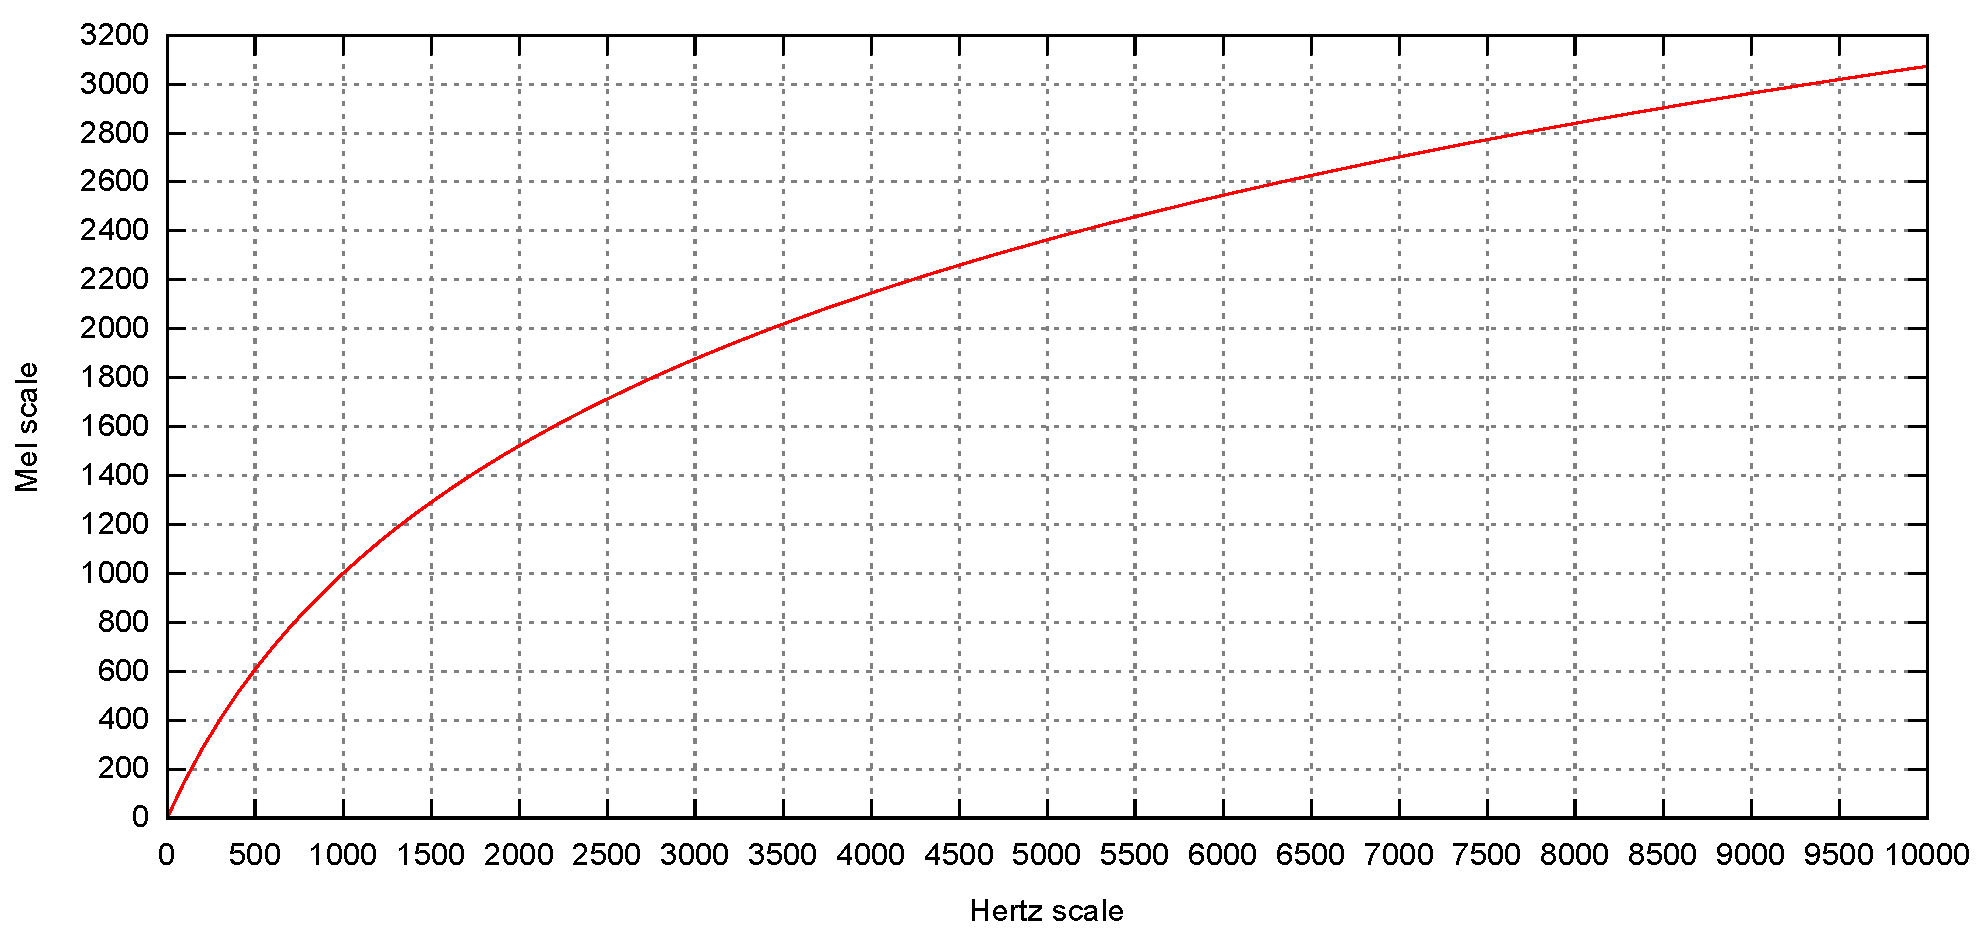
\includegraphics[width=\linewidth]{figures/Mel-Hz_plot.pdf}
    \caption{Plots of pitch mel scale versus Hertz scale}
\end{figure}

With mel scale applied on frequency axis of spectrogram, we get mel-spectrogram, which is used as the training target in this experiment.

\subsection{Tacotron 2}

Tacotron 2 is a neural network architecture for speech synthesis directly from text. The system is composed of a recurrent sequence-to-sequence feature prediction network that maps character embeddings to mel-scale spectrograms, followed by a modified WaveNet model acting as a vocoder to synthesize time-domain waveforms from those spectrograms. The architecture is illustrated in figure~\ref{figure:t2-block}

\begin{figure}[htb]
    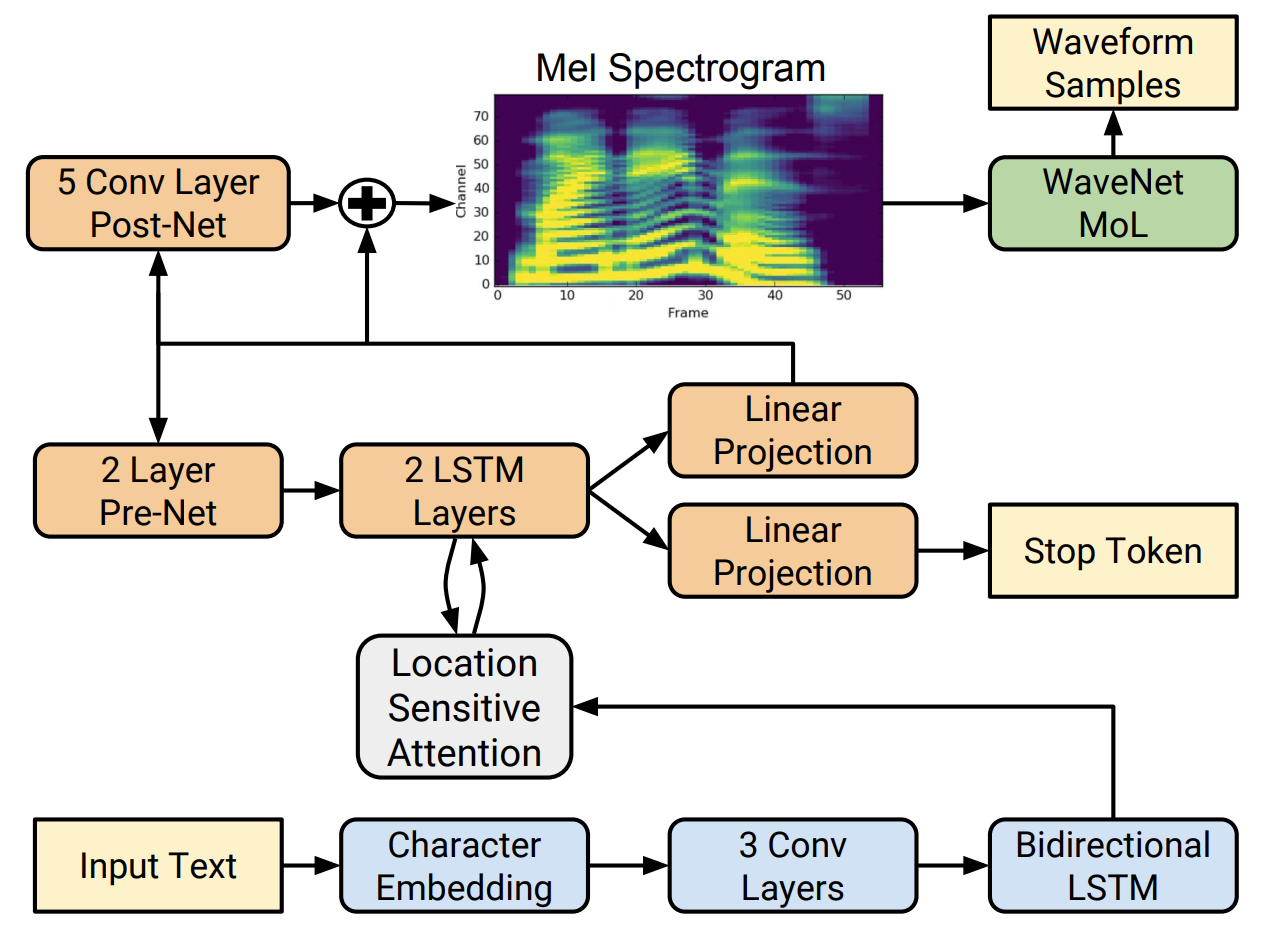
\includegraphics[width=\linewidth]{figures/t2-block.png}
    \caption{Block diagram of the Tacotron 2 system rchitecture}
    \label{figure:t2-block}
\end{figure}

\section{Experiments}

\subsection{Dataset}

we use the public speech synthesis dataset \emph{LJSpeech}\footnote{https://data.keithito.com/data/speech/LJSpeech-1.1.tar.bz2}. It consists of 13,100 short audio clips. A transcription is provided for each clip. Clips have a total length of approximately 24 hours.

\subsection{Implementation}

The whole pipeline is Implemented by Python, the model is based on \emph{PyTorch}, \emph{librosa} and some other packages are used to deal with audio signals.

I directly used the provided code. But that code is not well written, and contains some bugs. I made some small changes, and the synthesis improved dramatically. Due to the limited time and computation resources, I didn't perform the training process. But instead, I just used the provided checkpoint to run inference.

\subsection{Results}

Due to the limited time, I don't have many thing to report here. The synthesis quality is acceptable, when I listen to it, I can understand the content. But it contains many noise. So I suspect there are more bugs in the pipeline. I believe \emph{Tacotron 2} can perform better if Implemented correctly.

\section{Conclusion}

This experiment gives barely acceptable results. The well-known \emph{Tacotron 2} model can synthesis speech from any English sentences. In this experiment, I'm familiarised with the speech signal processing pipeline and the \emph{Tacotron 2} model. And my engineering skills are improved.

\end{document}
